\documentclass[conference]{IEEEtran}

\usepackage{amsmath,amssymb,amsfonts}
\usepackage{booktabs}
\usepackage{cite}
\usepackage{graphicx}
\usepackage{textcomp}
\usepackage{xcolor}
\usepackage{url}
\usepackage{xspace}
\usepackage[section]{placeins}
\usepackage[hidelinks]{hyperref}

\graphicspath{{assets/paper/}}

\newcommand{\modelname}{Simamba\xspace}
\newcommand{\mamba}{Mamba\xspace}
\newcommand{\mambatwo}{Mamba--2\xspace}
\newcommand{\mambathree}{Mamba--3\xspace}
\newcommand{\appendixwidefigure}[3]{%
\begin{figure*}[p]
    \centering
    \includegraphics[width=0.82\textwidth]{#1}
    \caption{#2}
    \label{#3}
\end{figure*}
}
\newcommand{\appendixsmallfigure}[3]{%
\begin{figure*}[p]
    \centering
    \includegraphics[width=0.68\textwidth]{#1}
    \caption{#2}
    \label{#3}
\end{figure*}
}
\newcommand{\appendixrunfigure}[3]{%
\begin{figure*}[p]
    \centering
    \includegraphics[width=0.82\textwidth]{#1}
    \caption{#2}
    \label{#3}
\end{figure*}
}

\begin{document}

\title{\modelname: Evaluating Simpson-Style Discretization for Mamba--3 State Space Language Models}

\author{
\IEEEauthorblockN{Soumil Baldota, Ansen Shia, and David Zhang}
\IEEEauthorblockA{
\textit{School of Engineering and Applied Sciences}\\
\textit{Columbia University}\\
New York, NY, USA\\
\{ssb2234, as8008, dwz2107\}@columbia.edu
}
}

\maketitle

\begin{abstract}
State space sequence models offer linear-time alternatives to Transformer attention, but their quality and stability depend strongly on the numerical discretization used to update recurrent state. This project studies whether a Simpson-style update can improve the SISO-style recurrence path in our \mambathree-inspired repository implementation. We implement \modelname, a mixer that replaces the matched trapezoid state update with a learned width-3 Simpson recurrence, and we build the end-to-end training, evaluation, checkpointing, benchmarking, and Hugging Face/vLLM export pipeline needed to test it. On a single Tesla V100, we train controlled 10M-parameter language models on SlimPajama subsets with fixed validation sampling, no-replacement training sampling, AdamW, cosine learning-rate decay, fp32 parameter storage, and gradient health logging. The final controlled runs are stable, but the current Simpson parameterization does not consistently outperform the baselines: it does not beat \mambatwo, and the matched trapezoid controls remain stronger in the 50M-token ablations. In the long-run 500M+ comparison, Simpson+midpoint reaches best validation loss 4.9178 versus 4.8625 for \mambatwo and 4.9326 for matched trapezoid, but at different training steps. The systems result is mixed: the original repository benchmark has decode-step latency within about 8\% of \mambathree but prefill hundreds of times slower, while the current repo adds a forward-only improved prefill kernel and profiling harness that still need end-to-end serving validation. The main contribution is therefore a reproducible negative result and a diagnosis: Simpson's negative lag-2 correction is mathematically plausible but currently harder to optimize than the trapezoid update.
\end{abstract}

\begin{IEEEkeywords}
state space models, Mamba, language modeling, discretization, Simpson's rule, vLLM, GPU training
\end{IEEEkeywords}

\section{Introduction}

Selective state space models (SSMs), especially the \mamba family, replace quadratic attention with linear-time recurrent scans while preserving strong language-modeling quality \cite{mamba,mamba2}. The latest \mambathree line adds inference-first SSM dynamics and specialized kernels; this project targets the SISO-style recurrence path used in our repository implementation \cite{mamba3}. This exposes a numerical question that Transformers avoid: how should a continuous-time SSM be discretized into a stable, trainable, GPU-efficient recurrence? Thus, we hypothesize that a Simpson-style state update (being a higher-order method than the trapezoidal rule for smooth functions) could better approximate the forcing term in a selective SSM and thereby improve language model performance. We refer to the resulting mixer as \modelname. This variant retains the \mambathree SISO interface, projections, rotary state, skip path, and language model wrapper, but replaces the width-2 trapezoid recurrence with a width-3 Simpson-inspired update.

Due to reliability issues with the intended multi-GPU A6000 Slurm environment, the study was carried out on a single V100 instead. This limitation turned the study into a controlled negative result rather than a scaling claim: once gradient instability, checkpointing, validation sampling, and memory pressure were addressed, Simpson-style dynamics trained stably but did not consistently outperform \mambatwo or the matched \modelname trapezoid baseline. Overall, our results suggests that the learned negative lag-2 Simpson term is the primary optimization bottleneck. This highlights how the reparameterization challenge that must be addressed before scaling up training.

\section{Literature Review}

\subsection{Selective State Space Models}

An SSM layer models a sequence through a recurrent state. Mathematically, in simplified continuous time the dynamics are described as follows:
\begin{align}
    \frac{d h(t)}{dt} &= A(t)h(t) + B(t)x(t),\\
    y(t) &= C(t)h(t)+D(t)x(t),
\end{align}
where the Mamba family makes the dynamics selective by allowing input-dependent parameters \cite{mamba}. The following iteration, \mambatwo, reformulates the computation using structured state space duality and a hardware-efficient chunk scan \cite{mamba2}. Finally, the recent \mambathree paper submitted in March emphasizes inference-first SSM dynamics; our repository implementation exposes a SISO-style path with token-dependent query/key/value-like streams and recurrent state updates \cite{mamba3}.

In the language models used here, the recurrent state can be written as a head-wise matrix $H_t$ driven by a value-key outer product:
\begin{equation}
    X_t = v_t k_t^\top,\qquad y_t = H_t q_t + Dv_t,
\end{equation}
where $q_t$, $k_t$, and $v_t$ are generated by a learned input projection and rotary state. The discretization determines how $X_t$ and previous $X_{t-i}$ terms enter $H_t$.

\subsection{Why Simpson's Rule Was Worth Testing}
\begin{figure*}[t]
    \centering
    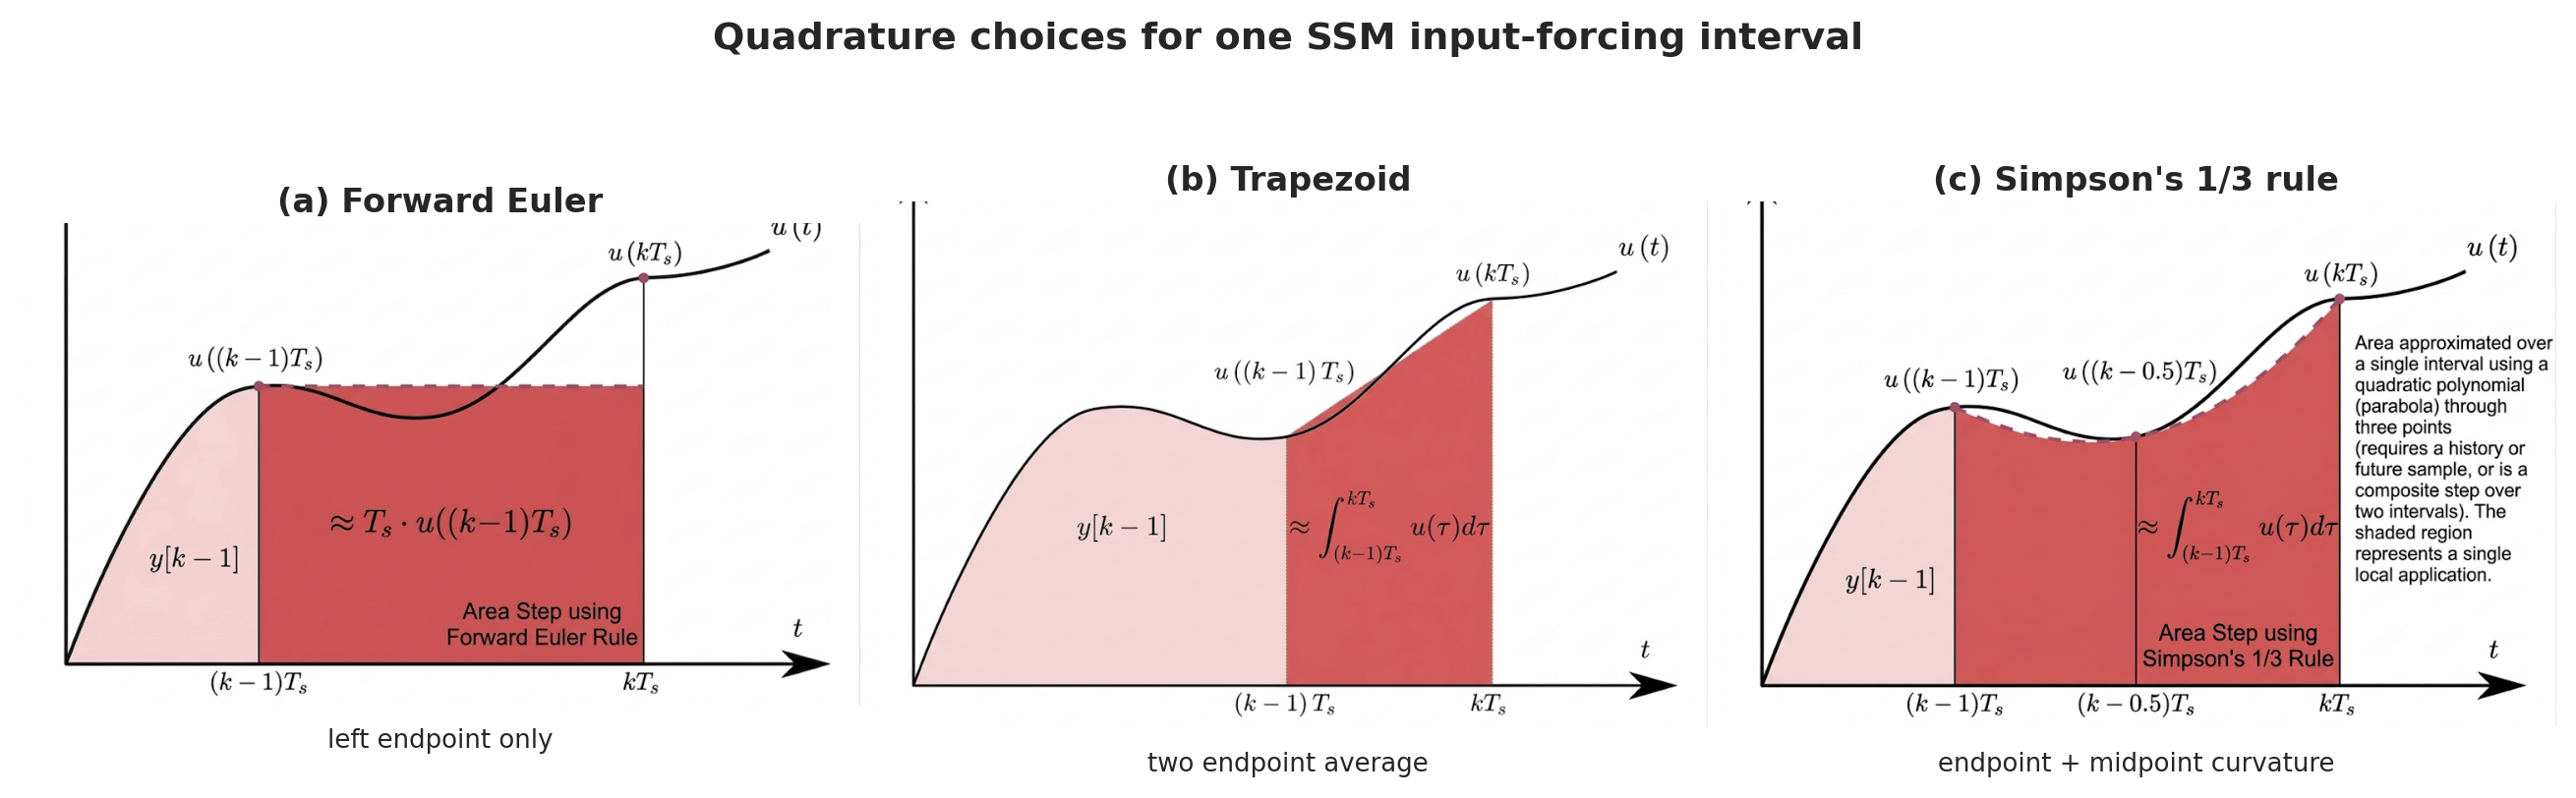
\includegraphics[width=0.98\textwidth]{discretization_comparison.png}
    \caption{Discretization intuition from the provided quadrature diagrams. Euler uses only the left endpoint, trapezoid averages the two endpoints, and Simpson's rule adds a midpoint/curvature term. \modelname uses this last idea as a causal learned width-3 SISO update, which introduces the negative lag-2 correction studied in the experiments.}
    \label{fig:discretization_visual}
\end{figure*}
For a scalar linear ODE with a forcing term, the exact discrete update involves an integral over the interval. Trapezoidal integration approximates this integral using only the endpoints, whereas Simpson’s rule also incorporates the midpoint, giving a higher-order approximation for smooth forcing functions. Figure~\ref{fig:discretization_visual} illustrates this quadrature intuition. However, in a language-model SSM, the forcing term is a token-dependent value-key product $v_tk_t^\top$, rather than a smooth scalar signal. As a result, the Simpson argument provides motivation but does not guarantee a better recurrence. To remain causal and GPU-efficient, \modelname encodes midpoint and curvature information via a learned, history-only width-3 correction, rather than relying on a noncausal future sample. Our experiments examine whether this numerical intuition holds up under optimization in a learned model.

\section{Methodology}

\subsection{Architecture}

Fig.~\ref{fig:arch} compares \modelname with the repository Mamba--2 and Mamba--3 block diagrams. The language model embeds token IDs, applies residual RMSNorm mixer blocks, and uses a tied LM head. \modelname keeps the Mamba--3-style projection, RoPE state, skip path, gate, and output projection, but replaces the internal SISO transform with the Simpson recurrence to better capture midpoint and curvature information in the dynamics. Each hidden state is projected into $z_t$, $x_t$, $B_t$, $C_t$, $\Delta_t$, $A_t$, discretization controls, and rotary-angle parameters before the recurrence and output path, helping ensure that the model can flexibly adapt its numerical integration while preserving causality and GPU efficiency. Overall, our approach aims to combine the higher-order precision of Simpson-style updates while retaining the established stability of the \mambathree baseline.

\begin{figure*}[t]
    \centering
    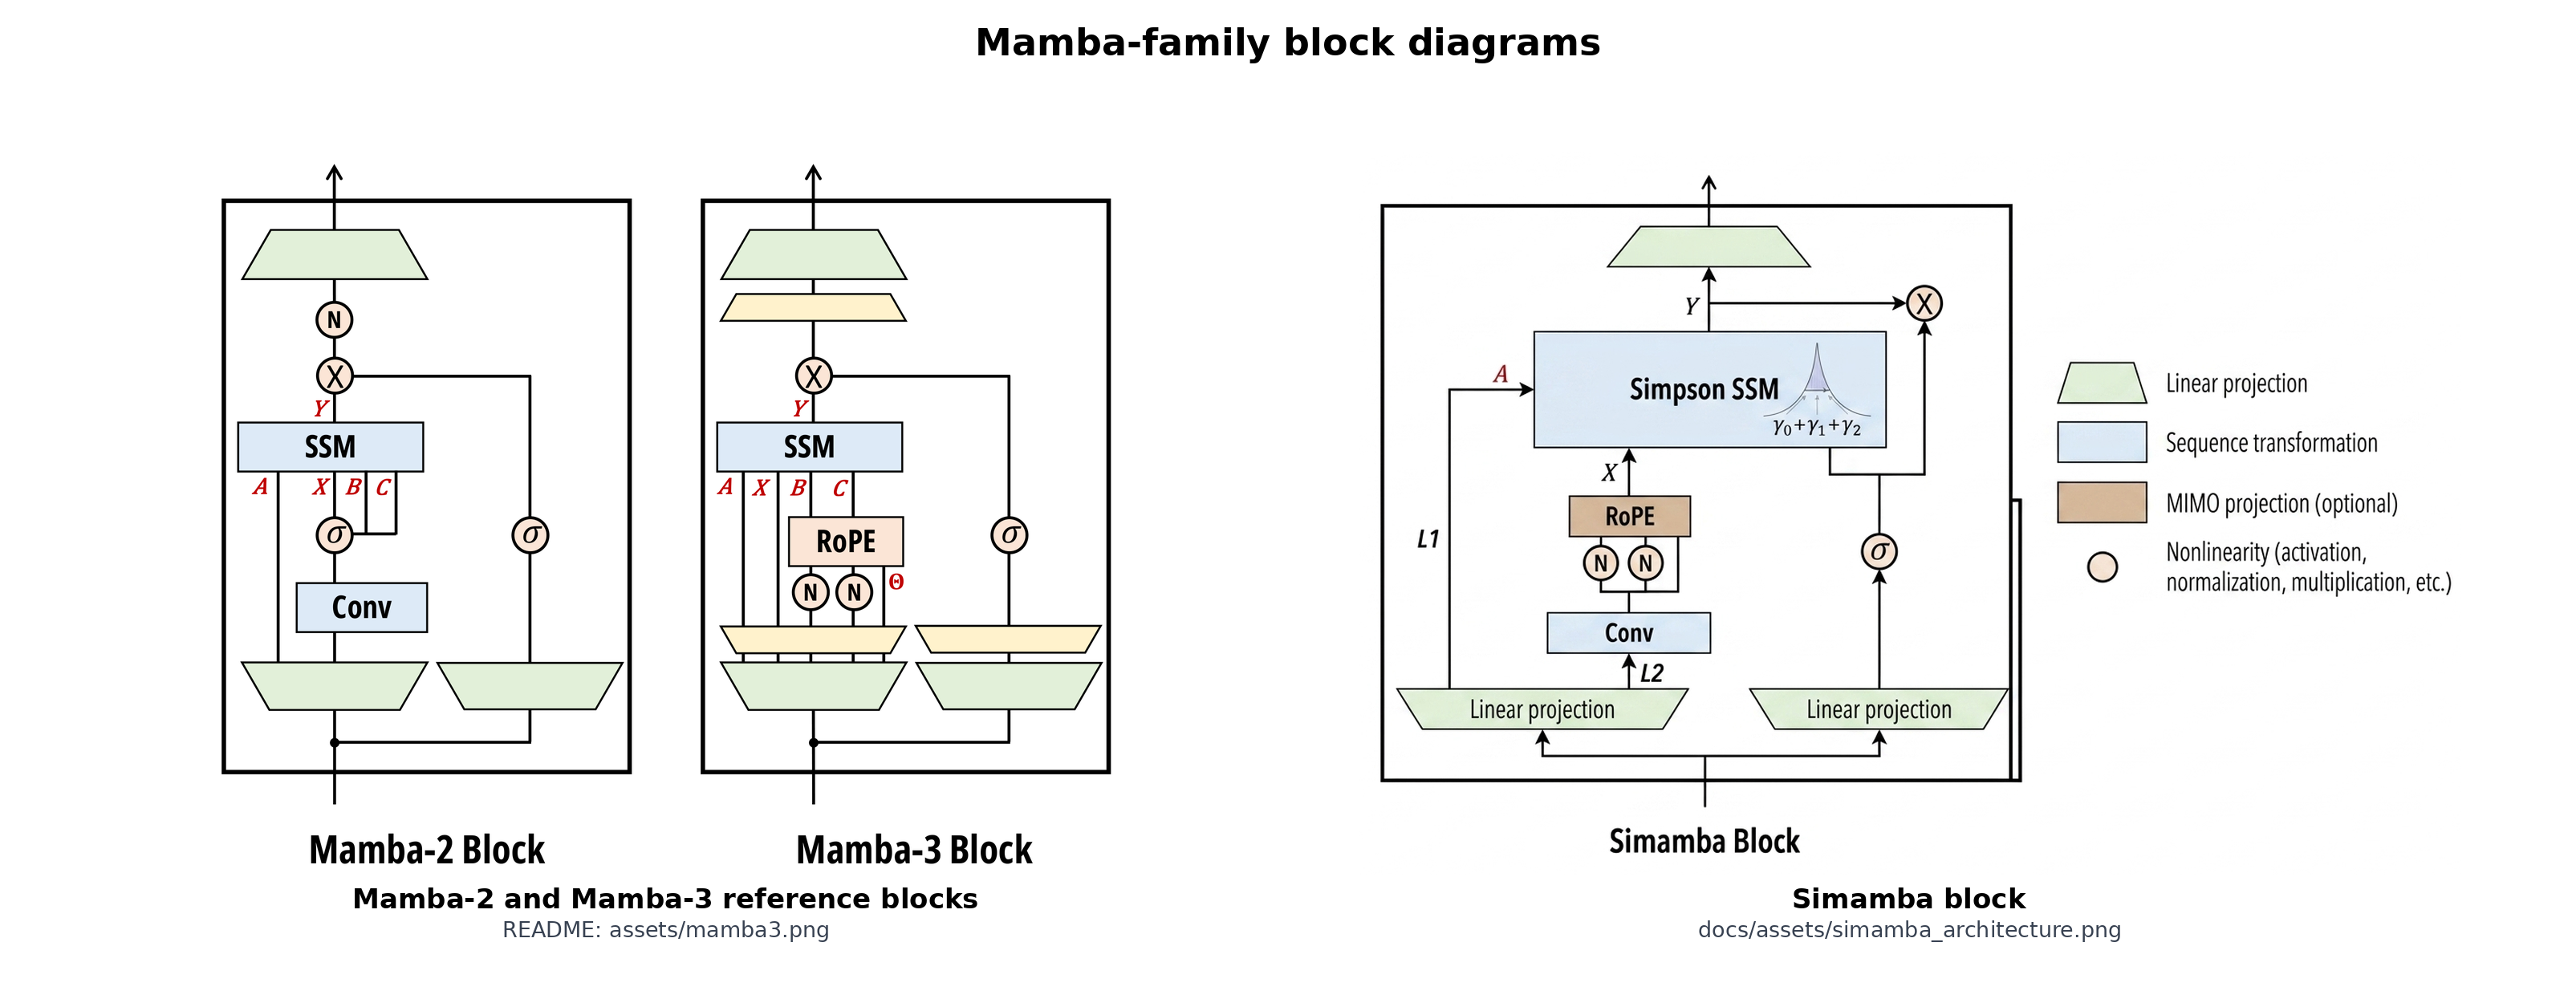
\includegraphics[width=0.95\textwidth]{mamba_family_architecture_comparison.png}
    \caption{Architecture comparison using the README Mamba--2/Mamba--3 block diagram and the added \modelname block diagram. \modelname preserves the Mamba--3-style block skeleton but changes the sequence transformation to a Simpson SSM. The matched trapezoid baseline uses the same projections, biases, rotary state, $D$ skip, and output path; only the SISO state-update coefficients change.}
    \label{fig:arch}
\end{figure*}

\subsection{Experimental Scope and Model Setup}

The optimization scope is both training and inference: training experiments evaluate whether Simpson discretization improves language-model validation loss, while inference experiments evaluate prefill, decode, memory, kernel traces, and vLLM serving behavior \cite{vllm}. All controlled language-model experiments use a 10M-parameter decoder-only \texttt{MambaLMHeadModel} with 8 layers, $d_{\mathrm{model}}=160$, sequence length 128, tied embeddings, fp32 residuals/parameters, and a 50,280-token GPT-NeoX vocabulary. For \modelname, each mixer expands to $d_{\mathrm{inner}}=320$, uses 10 heads of dimension 32, and uses SISO state dimension 64. Training uses micro-batch 8, gradient accumulation to global batch 64, and chunk size 16. Simpson, Simpson + midpoint, and matched trapezoid variants share the same projection and output path; local-conv variants add width-4 causal depthwise mixing over the $x/B/C$ stream.

\subsection{Matched Trapezoid Baseline}

The comparison baseline is not stock \mambatwo. Because \mambatwo incorporates a causal local convolution and a different parameterization, it does not serve as a pure discretization control. To provide a fair comparison, we implemented a matched \modelname trapezoid path using the same projection layout as \modelname. Let
\begin{equation}
    \alpha_t=\exp(A_t\Delta_t), \qquad p_t = \sigma(c_t),
\end{equation}
where $c_t$ is the learned trapezoid coefficient logit. The vectorized training form uses a width-2 contribution:
\begin{equation}
    \gamma_t = \Delta_t p_t,\qquad
    s_t = \gamma_t + \Delta_{t+1}(1-p_{t+1}),
\end{equation}
and updates the recurrent state in simplified form as
\begin{equation}
    H_t = \alpha_t H_{t-1} + s_t(v_tk_t^\top).
\end{equation}
This construction ensures that the trapezoid baseline matches \modelname in all architectural aspects except for the internal recurrence rule, so any performance differences can be attributed to the discretization method itself. Rotary state, $Q/K$ biases, $D$ skip, optional $z$ gate, and fixed boundary handling are preserved to maintain consistency, ensuring that the baseline remains a controlled test of whether Simpson-style updates provide a meaningful numerical advantage.

\subsection{Simpson-Style Update}

\modelname{} replaces the trapezoid contribution with a learned width-3 Simpson-like recurrence. Define
\begin{equation}
    \alpha_t = \exp(A_t\Delta_t), \qquad
    \alpha_{t,1/2} = \exp(A_t\Delta_t/2),
\end{equation}
and a bounded learned Simpson correction
\begin{equation}
    s_t = \mathrm{clip}(\sigma(c_t)m_t,0,1),
\end{equation}
where $m_t=1$ unless midpoint control is enabled, in which case $m_t=\sigma(r_t)$ is learned from an additional projection. The coefficients are
\begin{align}
    \gamma_{0,t} &= \frac{\Delta_t}{6}\left(1+\alpha_{t,1/2}(2-\frac{1}{2}s_t)\right),\\
    \gamma_{1,t} &= \frac{\Delta_t}{6}\left(\alpha_t+\alpha_{t,1/2}(2+s_t)\right),\\
    \gamma_{2,t} &= -\frac{\Delta_t}{12}\alpha_{t,1/2}s_t .
\end{align}
The state update is
\begin{equation}
\begin{split}
H_t ={}& \alpha_t H_{t-1}
    + \gamma_{0,t}(v_tk_t^\top)
    + \gamma_{1,t}(v_{t-1}k_{t-1}^\top)\\
    &+ \gamma_{2,t}(v_{t-2}k_{t-2}^\top).
\end{split}
\label{eq:simpson}
\end{equation}
The negative lag-2 term $\gamma_{2,t}$ is the key distinction from the trapezoid update. It also appears to be the primary contributor to the noisier gradient norms observed in Appendix Fig.~\ref{fig:app_main_grad}. To mitigate potential instability, we introduced two safeguards: a coefficient logit offset that initializes $s_t$ closer to zero, and an optional midpoint control that reduces the effective correction when needed. These controls allow the model to benefit from higher-order Simpson-style updates while maintaining stable training dynamics.

Intuitively, Simpson-style weighting can better capture the curvature of the forcing term over the interval by incorporating information from the midpoint in addition to the endpoints. In the language-model setting, where the forcing term is a token-dependent value-key product rather than a smooth scalar, the learned width-3 recurrence provides a flexible mechanism to approximate this curvature. By encoding history-dependent corrections, \modelname{} can potentially improve the fidelity of the state update compared to the simpler trapezoid rule, aligning numerical intuition with practical, trainable dynamics.

\subsection{Implementation and Evaluation Protocol}

The implementation adds the \texttt{Simamba} mixer, reference and Triton Simpson SISO operators, matched trapezoid controls, local-convolution controls, checkpoint/resume metadata, fixed validation sampling, and profiling scripts. The trainable Triton path exposes the Simpson recurrence through a PyTorch autograd wrapper, while a separate forward-only improved prefill kernel is used for systems profiling. The best \modelname and \mambatwo checkpoints were exported to Hugging Face, with the improved profiling export hosted at \url{https://huggingface.co/kalcy0n/improved-simamba-10m-slimpajama-500m}. Additional implementation details are moved to the appendix.

We use SlimPajama \cite{slimpajama}, streamed from Hugging Face with the GPT-NeoX tokenizer \cite{gptneox}, EOS-appended documents, and \texttt{uint16} token memory maps. The primary prepared split contains 500M train tokens from 691,532 documents and 50M validation tokens from 49,451 documents; the matched 50M experiments draw budgets from the same prepared data. The final reported runs use one NVIDIA Tesla V100-SXM2 16GB after the intended multi-GPU A6000 Slurm environment proved unreliable. Training uses AdamW \cite{adamw}, linear warmup plus cosine decay, gradient clipping at 1.0, fp32 parameter storage, fixed validation spans, no-replacement epoch sampling, nonfinite-step detection, and W\&B logging of configuration, train/validation loss, gradient norms, learning rate, throughput, and memory/profiling summaries.

\section{Experimental Results}

The public W\&B dashboard contains the reported runs. For reproducible paper generation without requiring API credentials, the plotting script also reconstructs figures from locally synchronized W\&B logs and JSON metric records.

\subsection{Initial Instability}

Early runs exhibited unstable gradients before warmup completed; while clipping kept the post-clip updates bounded, it masked large pre-clip norms. Appendix Fig.~\ref{fig:app_initial_instability} shows a representative example of this behavior. The controlled runs became stable after switching to fp32 parameters, adding cosine decay, lowering peak learning rates, and logging nonfinite-step/checkpoint metadata.

\begin{figure*}[t]
    \centering
    \begin{minipage}{0.32\textwidth}
        \centering
        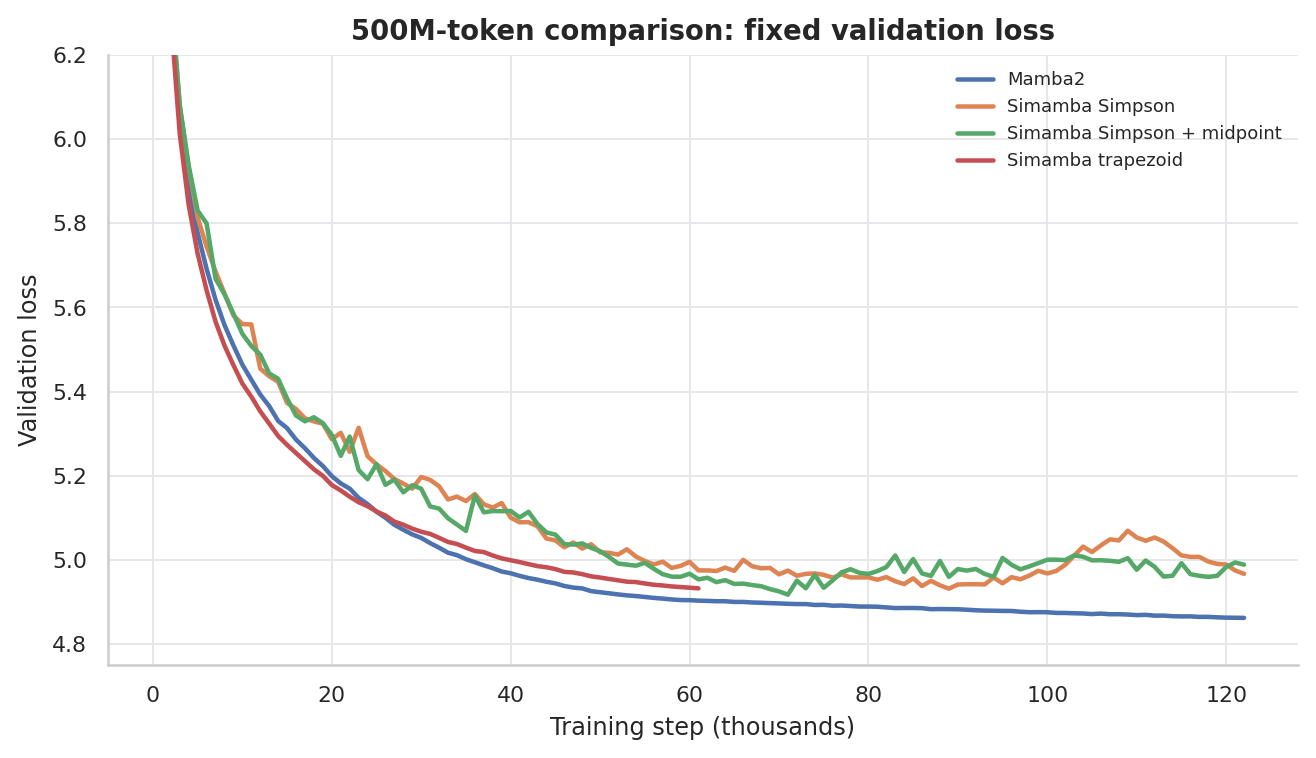
\includegraphics[width=\linewidth]{wandb_main_500m_val_loss.png}\\
        \scriptsize 500M-token comparison
    \end{minipage}\hfill
    \begin{minipage}{0.32\textwidth}
        \centering
        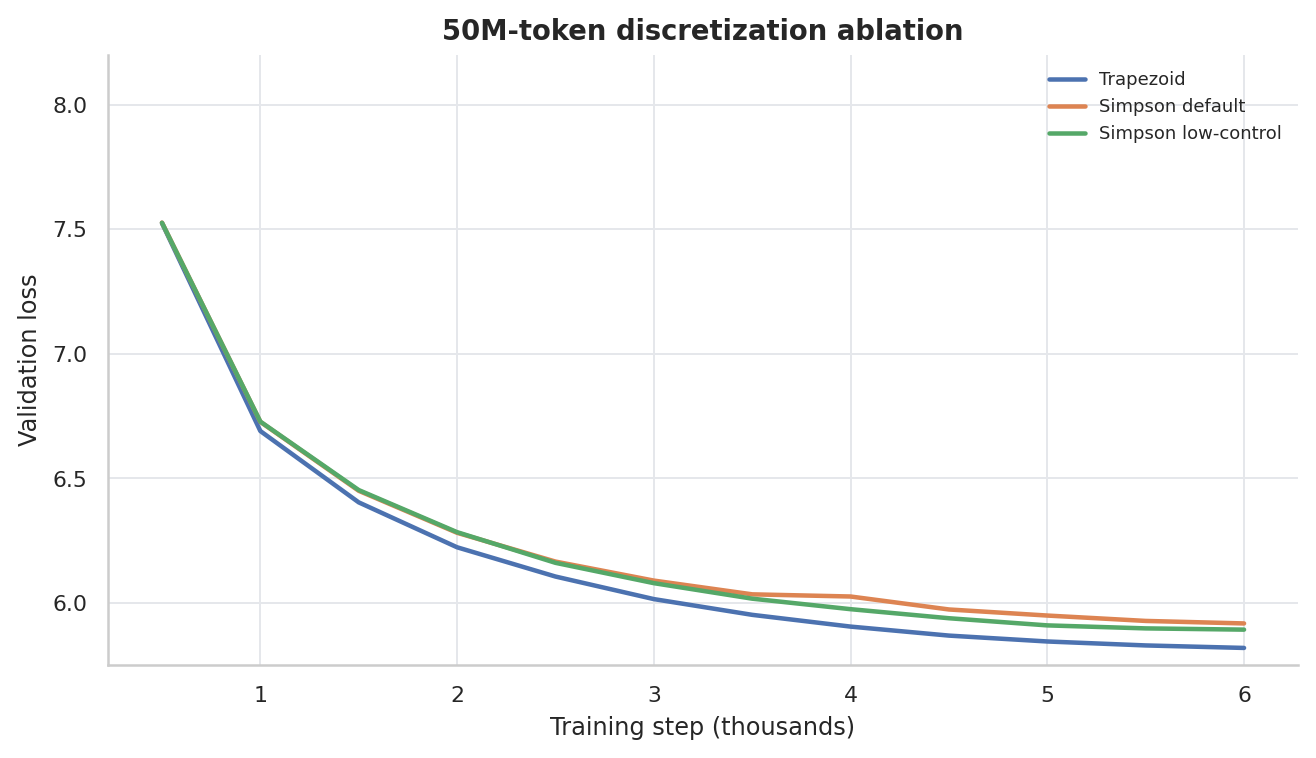
\includegraphics[width=\linewidth]{wandb_50m_discretization_val_loss.png}\\
        \scriptsize 50M discretization ablation
    \end{minipage}\hfill
    \begin{minipage}{0.32\textwidth}
        \centering
        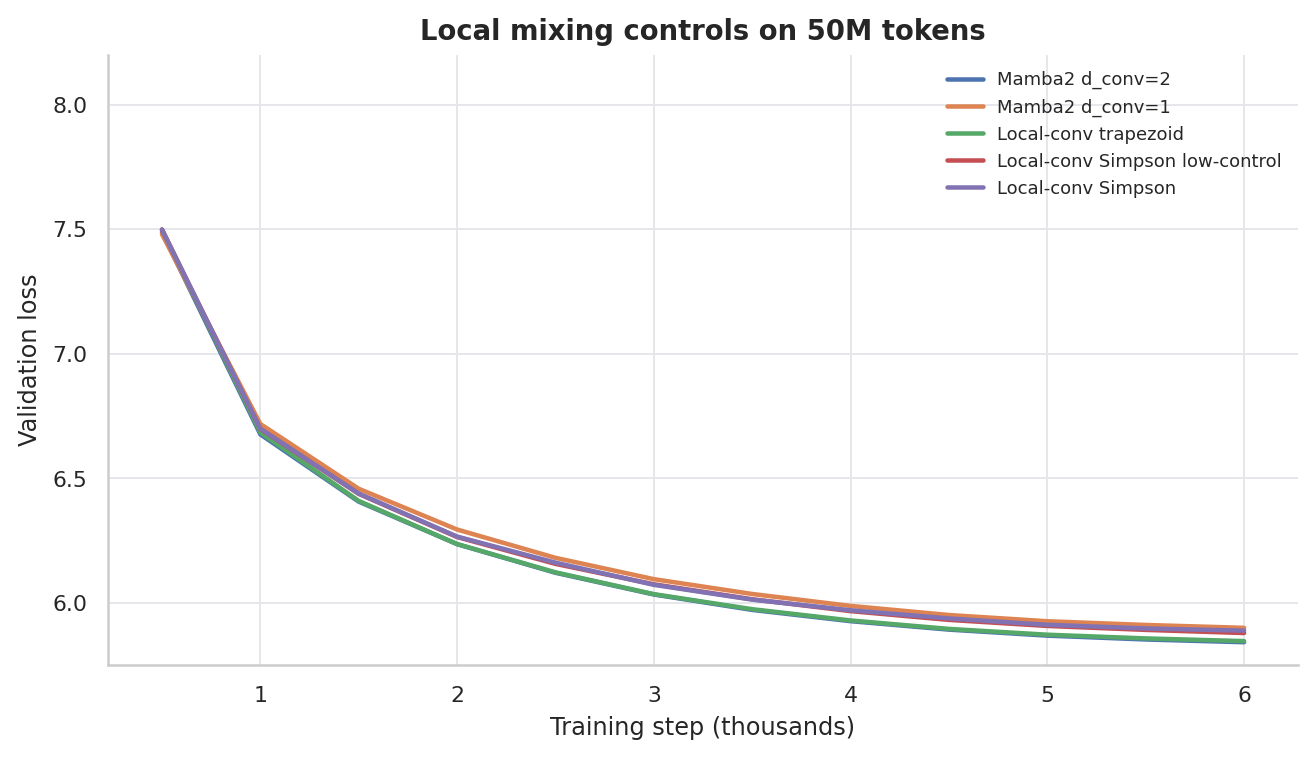
\includegraphics[width=\linewidth]{wandb_localmix_val_loss.png}\\
        \scriptsize Local-mixing control
    \end{minipage}
    \caption{Main validation-loss evidence. Across the long run, matched ablation, and local-convolution control, Simpson-style updates train stably but do not consistently outperform \mambatwo or the matched trapezoid controls.}
    \label{fig:main_validation_curves}
\end{figure*}

\subsection{Long-Run 500M+ Token Comparison}

The primary comparison starts from one 500M-token pass and then continues the main variants when useful. Table~\ref{tab:main} therefore reports best checkpoints from a long-run 500M+ comparison, not a strict equal-budget comparison. From Table~\ref{tab:main}, we observe that the best validation performance is roughly comparable across variants, with \mambatwo achieving 4.8625 and the Simpson-style and trapezoid variants slightly higher at 4.9178-4.9326. Notably, the Simpson variants tend to reach their best checkpoints later in terms of seen tokens, reflecting the slower training observed in Table~\ref{tab:train_health}. Model dimensions are $d_{\mathrm{model}}=160$, 8 layers, $d_{\mathrm{state}}=64$, head dimension 32, sequence length 128, and tied input/output embeddings.

\begin{table}[t]
\caption{Long-run 500M+ language-model comparison. Seen tokens are estimated as step count times the 8192-token global batch.}
\label{tab:main}
\centering
\scriptsize
\begin{tabular}{@{}lrrrrr@{}}
\toprule
Model & Best val. & Step & Seen & Last val. & Last train\\
\midrule
\mambatwo & 4.8625 & 122k & 999M & 4.8625 & 4.2041\\
\modelname{} Simpson & 4.9319 & 89k & 729M & 4.9671 & 4.3852\\
\modelname{} Simpson+midpoint & 4.9178 & 71k & 582M & 4.9889 & 4.3816\\
\modelname{} trapezoid & 4.9326 & 61k & 500M & 4.9326 & 4.4823\\
\bottomrule
\end{tabular}
\end{table}

The validation curves in Fig.~\ref{fig:main_validation_curves} are the strongest evidence against the current Simpson formulation. The corresponding per-run charts are Figs.~\ref{fig:run-chart-main-500m-token-comparison-mamba2}--\ref{fig:run-chart-main-500m-token-comparison-simamba-trapezoid}. \mambatwo is the best overall model, but it is not a pure discretization baseline. More importantly, the matched \modelname trapezoid baseline is competitive with and slightly better than default Simpson, while Simpson+midpoint has a better best checkpoint but worse final validation.

\begin{table}[t]
\caption{Tail training throughput and gradient-health summary for the long-run models. Throughput is median tail tokens/s; gradient norm is median tail pre-clip norm.}
\label{tab:train_health}
\centering
\footnotesize
\begin{tabular}{@{}lrr@{}}
\toprule
Model & Tok/s & Grad. norm\\
\midrule
\mambatwo & 16.1k & 3.32\\
\modelname{} Simpson & 12.5k & 5.77\\
\modelname{} Simpson+midpoint & 12.6k & 5.16\\
\modelname{} trapezoid & 16.3k & 2.50\\
\bottomrule
\end{tabular}
\end{table}

Table~\ref{tab:train_health} highlights two practical observations from the long-run training experiments. First, the Simpson variants (\modelname{} Simpson and Simpson+midpoint) show reduced training throughput compared to \mambatwo and the matched trapezoid baseline, achieving roughly 12.5–12.6k tokens/s versus 16k tokens/s. Second, their tail pre-clip gradient norms are noticeably higher, with median values of 5.16–5.77 compared to 2.50–3.32 for the trapezoid and \mambatwo models. This is consistent with the noisier-gradient behavior illustrated in Appendix Fig.~\ref{fig:app_main_grad} and underscores the gradient sensitivity introduced by the negative lag-2 Simpson term. Together with the earlier observation of early-run instability (Appendix Fig.~\ref{fig:app_initial_instability}), these results suggest that while Simpson-style updates can be trained stably, they incur higher computational cost and gradient variance relative to simpler discretization schemes.

\subsection{Matched 50M-Token Discretization Ablation}

To reduce runtime and isolate the effect of discretization, we ran a 50M-token matched ablation using identical model size, data, batch size, seed, and training schedule across all variants. Table~\ref{tab:ablation50} summarizes the results. The trapezoid baseline achieves the best validation score of 5.8195 and a final training loss of 5.6111, establishing a strong reference. The default Simpson variant lags behind, with a best validation of 5.9178 and a final training loss of 5.7161. Lowering the initial Simpson correction improves performance slightly, yielding a best validation of 5.8929 and final training loss of 5.6995, but it still does not surpass the trapezoid baseline.

These results indicated to us that while reducing the Simpson correction mitigates some of the gradient noise, the width-3 recurrence alone does not provide a consistent numerical advantage at this scale. The corresponding validation curves in Fig.~\ref{fig:main_validation_curves} illustrate these trends across training, and the individual run charts (Figs.~\ref{fig:run-chart-matched-50m-token-discretization-ablation-trapezoid}–\ref{fig:run-chart-matched-50m-token-discretization-ablation-simpson-low-control}) further detail the per-step dynamics for each variant.

\begin{table}[t]
\caption{50M-token matched discretization ablation.}
\label{tab:ablation50}
\centering
\begin{tabular}{lrrr}
\toprule
Variant & Best/final val. & Last train & Skips\\
\midrule
Trapezoid & 5.8195 & 5.6111 & 0\\
Simpson default & 5.9178 & 5.7161 & 0\\
Simpson low-control & 5.8929 & 5.6995 & 0\\
\bottomrule
\end{tabular}
\end{table}

\subsection{Local-Convolution Confound}

\mambatwo includes a depthwise causal convolution over the $x/B/C$ stream before the SSM update. We initially had \modelname omit this component. This design choice proves important: as shown in Table~\ref{tab:local}, reducing or removing the convolution in \mambatwo degrades quality, with best validation scores rising from 5.8425 for \(d_{\mathrm{conv}}=2\) to 5.9001 for \(d_{\mathrm{conv}}=1\). To ensure a fair comparison and maintain similar local-mixing capacity, we added \texttt{--simamba-d-conv 4} to \modelname.

With this adjustment, we can see in Table~\ref{tab:local} the trapezoid variant of \modelname achieves a best validation of 5.8469, nearly matching \mambatwo with \(d_{\mathrm{conv}}=2\). Simpson-style variants with and without reduced control see slightly higher validation values (5.8793–5.8890), reflecting the combined effects of the higher-order recurrence and local-convolution control. These results confirm that local feature mixing is a critical component for model quality and that \modelname can leverage it effectively while experimenting with Simpson-style updates.

\begin{table}[t]
\caption{Local-mixing controls on 50M tokens.}
\label{tab:local}
\centering
\begin{tabular}{lrr}
\toprule
Variant & Best/final val. & Last train\\
\midrule
\mambatwo{} $d_{\mathrm{conv}}=2$ & 5.8425 & 5.6268\\
\mambatwo{} $d_{\mathrm{conv}}=1$ & 5.9001 & 5.6958\\
\modelname{} local-conv trapezoid & 5.8469 & 5.6309\\
\modelname{} local-conv Simpson low-control & 5.8793 & 5.6701\\
\modelname{} local-conv Simpson & 5.8890 & 5.6759\\
\bottomrule
\end{tabular}
\end{table}

The overlay in Fig.~\ref{fig:main_validation_curves} and the per-run charts in Figs.~\ref{fig:run-chart-local-mixing-control-mamba2-d-conv-2}--\ref{fig:run-chart-local-mixing-control-local-conv-simpson} show the same pattern. This experiment is important because it prevents a misleading \mambatwo-vs-\modelname conclusion. Some of \mambatwo's advantage comes from local mixing, not only from its state discretization. After matching that mechanism, Simpson still trails the matched trapezoid update.

\subsection{Throughput, Kernel, and Serving Evidence}

Training throughput on the V100 is summarized in Appendix Fig.~\ref{fig:app_throughput}. The non-local Simpson variants are slower than \mambatwo and trapezoid in the 500M runs, while the local-conv 50M runs are closer but still behind the fastest baselines.

The repository SISO benchmark evaluates prefill and decode separately. In the prefill phase, the original \modelname benchmark path is substantially slower than the \mambathree fused-kernel path, with slowdowns of 776.9$\times$ for B1/P128/G64 and 410.7$\times$ for B4/P1024/G256. In contrast, decode-step latency is much closer, with the original path being only about 1.08$\times$ slower. To avoid conflating these results, Table~\ref{tab:systems_summary} reports the \mambathree reference path, the original \modelname path, and the improved forward-only \modelname SISO prefill kernel separately. The vLLM table below, however, refers to the improved Hugging Face/vLLM export rather than the isolated kernel alone.

\begin{table}[t]
\caption{SISO systems evidence summary. Repository benchmark rows use B4/P1024/G256. NSYS rows use the B2/S256/H32/d64 kernel trace.}
\label{tab:systems_summary}
\centering
\scriptsize
\begin{tabular}{@{}lrrrl@{}}
\toprule
Measurement & \mambathree & \modelname & Impr. \modelname & Takeaway\\
\midrule
Repo prefill ms & 0.8602 & 353.3066 & -- & orig. slow\\
Repo decode ms/tok & 0.0160 & 0.0173 & -- & close decode\\
NSYS region ms & 1.883 & 8.457 & 0.937 & improved SISO\\
NSYS GPU ms & 0.811 & 7.034 & 0.453 & lower kernel work\\
\bottomrule
\end{tabular}
\end{table}

The old end-to-end-style SISO benchmark shows that \modelname decode is close to \mambathree, but unfortunately prefill is not competitive. However, the newer NSYS and NCU kernel profiles show that the improved prefill kernel resolves much of this isolated SISO bottleneck. For the B2/S256/H32/d64 configuration, the improved kernel achieves an NSYS region time of 0.937\,ms, compared with 1.883\,ms for the profiled \mambathree path and 8.457\,ms for the original \modelname kernel path. Summed CUDA GPU kernel time follows the same pattern: 0.453\,ms for the improved \modelname kernel, 0.811\,ms for \mambathree, and 7.034\,ms for the original \modelname implementation. The NCU profile supports the same conclusion. The improved kernel increases the L1/TEX cache hit rate to 86.76\% while reducing DRAM throughput to 3.77\%, indicating that the dominant bottleneck is no longer the severe memory-stall behavior observed in the initial custom kernel. Detailed profiler counters are provided in Appendix Tables~\ref{tab:app_nsys_kernel_profile} and \ref{tab:app_ncu_kernel_profile}.

The vLLM sweep in Appendix Table~\ref{tab:vllm_comparison} provides a more conservative evaluation because it measures complete exported models rather than only the isolated SISO scan. The improved \modelname export reduces peak GPU memory usage to 0.48--0.62$\times$ that of the exported \mambatwo model, although throughput remains lower, ranging from 0.38--0.87$\times$ of \mambatwo depending on prompt type and prefix-cache settings. Prefix caching highlights the strongest serving-side improvement. For repeated-prefix prompts, TTFT decreases from 23.40\,ms to 19.95\,ms for \mambatwo, whereas the improved \modelname export reduces TTFT from 29.05\,ms to 7.47\,ms. However, the worst-case configuration occurs for normal prompts with prefix caching enabled, where throughput drops to 131.4\,tok/s compared with 350.3\,tok/s for \mambatwo, while TTFT increases to 137.68\,ms. These results suggest that improving the SISO kernel alone is insufficient to optimize end-to-end serving performance. Other components, including projection layers, cache management, batching behavior, and prefix-cache execution paths, continue to dominate overall system efficiency.

Kernel correctness was checked against PyTorch reference implementations before interpreting these timings. The \mambathree kernel is checked against a Mamba--3/trapezoid PyTorch reference, while \modelname and the improved prefill kernel are checked against the Simpson PyTorch reference. The \mambathree and \modelname Triton kernels pass forward and backward checks on the small fp32 correctness configuration; the improved prefill kernel passes the forward output check, while its backward row is marked not applicable because the improved kernel is a forward-only prototype. Across passed checks, the worst absolute errors are $3.43\times10^{-5}$ for \mambathree, $1.53\times10^{-5}$ for \modelname, and $1.91\times10^{-6}$ for improved \modelname. Appendix Fig.~\ref{fig:app_kernel_correctness} summarizes the error scale.

The benchmark plots are provided in Appendix Figs.~\ref{fig:app_bench_latency}, \ref{fig:app_bench_throughput}, \ref{fig:app_bench_memory}, and \ref{fig:app_bench_ratio}. Collectively, these results demonstrate that the original prefill gap is a clear systems-level bottleneck rather than a consequence of model quality or validation loss. The improved prefill kernel significantly narrows this gap and validates the feasibility of efficient \modelname SISO execution. But while the improved prefill kernel substantially reduces the isolated SISO bottleneck and is promising, additional optimization at the full model-serving level is still required.

\subsection{Overall Result}

The overall conclusion is that the current Simpson-style recurrence is trainable and behaves consistently across settings, but it does not yet provide a clear advantage over strong baselines. The best \modelname Simpson checkpoint, the midpoint-control variant, reaches a validation loss of 4.9178, while the best overall language model remains \mambatwo at 4.8625. Across both the long-run 500M+ runs and the matched 50M-token ablations, the trapezoid controls remain highly competitive, suggesting that the benefit of higher-order discretization is, at this scale, comparable to simpler update rules rather than decisively better.

From a training perspective, Simpson variants show a distinct optimization profile: they tend to converge more slowly, exhibit higher gradient norms, and require additional stabilization mechanisms such as coefficient initialization offsets and optional midpoint control. These adjustments make training reliable, but they also indicate that the added recurrence complexity changes the optimization landscape in a meaningful way. This suggests that the current parameterization may not be the most efficient way to realize higher-order corrections in practice.

Side diagnostics on synthetic state tracking and compression are included in the appendix; neither changes the main negative result.

\section{Discussion}

\subsection{Why Simpson Underperformed}

The results suggest three interacting causes. First, Simpson's higher-order quadrature rationale assumes smooth forcing terms, but token-level language inputs are discontinuous and highly data dependent. Second, the learned negative lag-2 coefficient in (\ref{eq:simpson}) can produce cancellation and noisier gradients, especially early in training before the model has learned stable coefficients. Third, \mambatwo's local convolution is a major architectural confound; once we matched local mixing, Simpson improved but still did not beat trapezoid.

This does not prove that Simpson-style discretization is impossible for SSMs. It shows that the current direct parameterization is not enough. A better design may need a constrained positive decomposition, an annealed correction schedule, or a trust-region style bound on the lag-2 term.

\subsection{Systems Lessons}

The project also exposed a systems gap. Even if Simpson quality were better, the original prefill implementation would not be practical in production. The decode step is close to \mambathree, and the improved prefill kernel makes the isolated SISO scan competitive in the B2/S256/H32/d64 profile. The remaining systems work is end-to-end: fused projection layout, local convolution, recurrence, output projection, batching policy, and vLLM cache behavior all need to be measured together before claiming serving speedup. The V100 also lacks some newer Triton functionality used by \mambathree kernels, so a portable fallback path is needed for older GPUs.

\subsection{Limitations and Future Work}

The most important next steps are:
\begin{itemize}
    \item Reparameterize the Simpson correction so the negative lag-2 term cannot dominate early training.
    \item Anneal the Simpson coefficient from zero after the model has learned a stable trapezoid-like recurrence.
    \item Build a fused local-conv \modelname kernel and a V100-compatible benchmark fallback.
    \item Run multi-seed 50M-token comparisons only after a single-seed Simpson variant beats the matched trapezoid baseline.
    \item Evaluate on longer context lengths, where higher-order state updates may have a better chance to matter.
    \item Add finetuning-aware int4 and pruning experiments rather than one-shot perturbations.
    \item Integrate the custom \modelname remote-code path deeper into vLLM if the architecture becomes quality-positive.
\end{itemize}

\section{Conclusion}

We implemented and evaluated \modelname, a Simpson-style SISO discretization for \mambathree-inspired language models. The work establishes a fully reproducible pipeline on a single V100, including data preprocessing, training and evaluation loops, validation protocols, checkpointing, W\&B logging, compression analysis, benchmarking, and model export to serving frameworks. 

On the modeling side, the results are mixed but informative. Across controlled experiments, the Simpson recurrence does not consistently outperform \mambatwo or the matched trapezoid baseline. In the 50M-token ablations, the trapezoid variant is generally stronger, while in the 500M+ runs the Simpson-midpoint configuration achieves competitive best-checkpoint performance but does not retain a clear advantage at final validation. Overall, the evidence suggests that the benefits of the Simpson-style correction are not yet stable across training budgets or evaluation settings. 

Taken together, these findings indicate that Simpson-style updates are a viable but not yet dominant discretization choice in this setting. A promising direction for future work is to treat the Simpson correction as a constrained or annealed modification of a stable trapezoid recurrence, rather than as a full replacement, in order to better control optimization stability while preserving potential higher-order benefits.

\section*{Artifact Availability}

{\raggedright
The public project repository is
\href{https://github.com/hpmls26/simamba}{\texttt{github.com/hpmls26/simamba}}.
The public W\&B training dashboard is
\href{https://wandb.ai/ssb2234-columbia/simamba}{\texttt{wandb.ai/ssb2234-columbia/simamba}};
it contains tagged baseline and \modelname runs with model configuration,
train/validation loss, gradient norms, learning rate, throughput, GPU utilization
where available, GPU memory, hyperparameter/ablation sweep metadata, and run tags
separating baseline, Simpson, midpoint, trapezoid, and local-conv variants.
Profiling logs use the separate W\&B project \href{https://wandb.ai/ssb2234-columbia/profiling}{\texttt{wandb.ai/ssb2234-columbia/profiling}}. The best checkpoints are available as Hugging Face repositories
\href{https://huggingface.co/soumil1/simamba-midpoint-10m-slimpajama-500m}{\texttt{soumil1/simamba-midpoint-10m-slimpajama-500m}}
and \href{https://huggingface.co/soumil1/mamba2-10m-slimpajama-500m}{\texttt{soumil1/mamba2-10m-slimpajama-500m}}. The improved profiling export is
\href{https://huggingface.co/kalcy0n/improved-simamba-10m-slimpajama-500m}{\texttt{kalcy0n/improved-simamba-10m-slimpajama-500m}}. The local paper assets are generated by \texttt{scripts/generate\_hpml\_paper\_assets.py} and profiling statistics through \texttt{profiling/run\_all\_profiling.py}.
\par}


\begin{thebibliography}{00}
\bibitem{mamba}
A. Gu and T. Dao, ``Mamba: Linear-time sequence modeling with selective state spaces,'' arXiv:2312.00752, 2023.

\bibitem{mamba2}
T. Dao and A. Gu, ``Transformers are SSMs: Generalized models and efficient algorithms through structured state space duality,'' in \textit{Proc. International Conference on Machine Learning}, 2024.

\bibitem{mamba3}
A. Lahoti, K. Y. Li, B. Chen, C. Wang, A. Bick, J. Z. Kolter, T. Dao, and A. Gu, ``Mamba-3: Improved sequence modeling using state space principles,'' arXiv:2603.15569, 2026.

\bibitem{adamw}
I. Loshchilov and F. Hutter, ``Decoupled weight decay regularization,'' in \textit{Proc. International Conference on Learning Representations}, 2019.

\bibitem{slimpajama}
Cerebras Systems, ``SlimPajama: A 627B token cleaned and deduplicated version of RedPajama,'' Hugging Face dataset, 2023. [Online]. Available: \url{https://huggingface.co/datasets/cerebras/SlimPajama-627B}

\bibitem{gptneox}
S. Black, S. Biderman, E. Hallahan, Q. Anthony, L. Gao, L. Golding, H. He, C. Leahy, K. McDonell, J. Phang, M. Pieler, U. S. Prashanth, S. Purohit, L. Reynolds, J. Tow, B. Wang, and S. Weinbach, ``GPT-NeoX-20B: An open-source autoregressive language model,'' arXiv:2204.06745, 2022.

\bibitem{vllm}
W. Kwon, Z. Li, S. Zhuang, Y. Sheng, L. Zheng, C. H. Yu, J. Gonzalez, H. Zhang, and I. Stoica, ``Efficient memory management for large language model serving with PagedAttention,'' in \textit{Proc. ACM Symposium on Operating Systems Principles}, 2023.
\end{thebibliography}

\clearpage
\appendices
\section{AI Tool Use Disclosure}

Per the HPML AI Use Policy, this submission discloses AI assistance. The team used ChatGPT/Codex for codebase navigation, LaTeX editing, summarizing repository artifacts, consistency checking against generated figures/tables, and draft-review support on team-written material. Final profiling interpretations, performance reasoning, numerical analysis, and scientific conclusions were validated by the team using the repository, W\&B logs, profiler exports, and generated paper assets.

\clearpage
\section{Result Figures and Per-Run Charts}
\label{app:charts}

The main text keeps the result narrative and numerical tables close to the claims. The visual evidence is collected here so the results section is not interrupted by large chart exports. The aggregate figures include the instability trace (Fig.~\ref{fig:app_initial_instability}), main-run training loss (Fig.~\ref{fig:app_main_train}), gradient norms (Fig.~\ref{fig:app_main_grad}), best-loss summary (Fig.~\ref{fig:app_summary_best}), throughput summary (Fig.~\ref{fig:app_throughput}), repository SISO benchmark latency, throughput, memory, and ratio plots (Figs.~\ref{fig:app_bench_latency}, \ref{fig:app_bench_throughput}, \ref{fig:app_bench_memory}, and \ref{fig:app_bench_ratio}), vLLM serving plot (Fig.~\ref{fig:app_vllm_compare}), compression plot (Fig.~\ref{fig:app_compression}), and kernel-correctness plot (Fig.~\ref{fig:app_kernel_correctness}). The per-run figures below then show the same locally logged training histories as separate labelled charts for each reported run.

\subsection{Aggregate Result Figures}

\appendixwidefigure{wandb_initial_instability.png}{Initial unstable run. Gradient clipping held the post-clip update at 1.0, but the pre-clip norm stayed large and a nonfinite gradient was detected at step 159.}{fig:app_initial_instability}

\appendixwidefigure{wandb_main_500m_train_loss.png}{Smoothed training loss for the 500M-token comparison. All models learn the training distribution, so the validation gap is not caused by a broken data path.}{fig:app_main_train}

\appendixwidefigure{wandb_main_500m_grad_norm.png}{Smoothed pre-clip gradient norm. The Simpson variants show larger tail gradient norms than \mambatwo and the matched trapezoid run, consistent with harder optimization.}{fig:app_main_grad}

\appendixsmallfigure{summary_best_val_loss.png}{Best fixed validation loss across the controlled runs. Lower is better.}{fig:app_summary_best}

\appendixsmallfigure{wandb_training_throughput.png}{Median tail training throughput on the V100, computed from the last 100 logged W\&B points for each run.}{fig:app_throughput}

\appendixsmallfigure{simamba_latency.png}{Repository SISO benchmark latency. \modelname decode overhead is small, but the prefill implementation is not competitive without fused-kernel work.}{fig:app_bench_latency}

\appendixsmallfigure{simamba_throughput.png}{Repository SISO benchmark throughput. The current prefill gap is a systems bottleneck independent of validation loss.}{fig:app_bench_throughput}

\appendixsmallfigure{simamba_memory.png}{Repository SISO benchmark memory use. Memory is not the main bottleneck relative to the observed prefill-latency gap.}{fig:app_bench_memory}

\appendixsmallfigure{simamba_ratio_summary.png}{Repository SISO benchmark ratio summary comparing \modelname with the reference \mambathree path.}{fig:app_bench_ratio}

\appendixsmallfigure{vllm_mamba2_vs_improved_report.png}{vLLM serving comparison between the exported \mambatwo checkpoint and the improved \modelname export. Improved \modelname uses less peak GPU memory but remains slower in overall throughput, with a favorable TTFT result only for repeated-prefix prompts with prefix caching enabled.}{fig:app_vllm_compare}

\appendixsmallfigure{compression_loss_delta.png}{Validation loss delta after post-training perturbations. Int8 row-wise quantize-dequantize is nearly lossless; int4 and larger pruning ratios require finetuning or better kernels.}{fig:app_compression}

\appendixsmallfigure{kernel_correctness_errors.png}{Kernel correctness error scale of \mambathree and \modelname against their respective PyTorch references (Trapezoid and Simpson) for forward and backward checks. The improved \modelname row includes the forward check only because the improved prefill kernel only performs the forward pass, resulting in smaller errors}{fig:app_kernel_correctness}

\FloatBarrier
\clearpage
\subsection{Additional Implementation Details}

The main code paths are \texttt{simamba.py} for the mixer and inference-cache hooks, \texttt{simamba\_siso\_combined.py} for reference/vectorized Simpson and trapezoid updates, \texttt{mamba3\_siso\_fwd.py} and \texttt{mamba3\_siso\_bwd.py} for Triton kernels, \texttt{train\_simamba\_lm.py} for training/resume/evaluation, \texttt{prepare\_slimpajama.py} for token memmaps, and \texttt{scripts/generate\_hpml\_paper\_assets.py} for reproducible figures. The trainable PyTorch path wraps the Triton SISO recurrence in a custom autograd function, recomputes chunk-start states for the backward pass to reduce activation storage, and keeps a reference path for correctness checks and unsupported edge cases.

The native vLLM fork registers \texttt{SimambaForCausalLM}, maps exported fused projection weights into the vLLM module layout, and stores the Simpson recurrent state, rotary-angle state, and key/value history in the Mamba cache. The optimized single-request decode path uses a fused input projection and persistent per-layer recurrent state when prefix caching is disabled; prefix-cache mode uses the conservative cache-all path for correctness. The improved prefill kernel is currently a forward-only profiling artifact, so serving claims in the main text are limited to measured vLLM behavior and isolated SISO-kernel profiles.

\subsection{Kernel Profiling Tables}

\begin{table*}[t]
\caption{Nsight Systems SISO forward trace at $B=2$, $L=256$, 32 heads, and head dimension 64 on the Tesla V100-SXM2. Region is the profiled NVTX range. GPU time sums CUDA GPU kernel durations inside the range. Slowdowns are relative to the improved \modelname trace.}
\label{tab:app_nsys_kernel_profile}
\centering
\footnotesize
\begin{tabular}{@{}lrrrrrrr@{}}
\toprule
Path & Region & GPU time & Kernels & Launch API & Sync API & Region slow. & GPU slow.\\
 & ms & ms &  & $\mu$s & $\mu$s &  & \\
\midrule
\modelname{} improved & 0.937 & 0.453 & 4 & 66.3 & 112.7 & 1.00$\times$ & 1.00$\times$\\
\mambathree{} reference & 1.883 & 0.811 & 2 & 81.0 & 686.2 & 2.01$\times$ & 1.79$\times$\\
\modelname{} original & 8.457 & 7.034 & 7 & 122.9 & 6860.5 & 9.03$\times$ & 15.53$\times$\\
\bottomrule
\end{tabular}
\end{table*}

\begin{table*}[t]
\caption{vLLM comparison between the exported \mambatwo checkpoint and the improved \modelname export. Memory ratio is peak GPU memory divided by \mambatwo.}
\label{tab:vllm_comparison}
\centering
\footnotesize
\begin{tabular}{@{}llrrrrrrr@{}}
\toprule
Prompt & Cache & \mambatwo & Improved & Mem & \mambatwo & Improved & \mambatwo & Improved\\
 &  & tok/s & tok/s & ratio & TTFT ms & TTFT ms & TPOT ms & TPOT ms\\
\midrule
Normal & off & 344.1 & 298.1 & 0.62 & 23.25 & 28.93 & 2.214 & 2.493\\
Normal & on & 350.3 & 131.4 & 0.48 & 23.96 & 137.68 & 2.148 & 3.382\\
Repeated & off & 350.2 & 256.8 & 0.62 & 23.40 & 29.05 & 2.195 & 2.593\\
Repeated & on & 365.2 & 288.2 & 0.48 & 19.95 & 7.47 & 2.169 & 3.331\\
\bottomrule
\end{tabular}
\end{table*}

\begin{table*}[t]
\caption{Nsight Compute isolated SISO kernel profile for the same $B=2$, $L=256$, 32-head, head-dimension-64 setup. Time is instrumented per-launch kernel time from NCU; improved \modelname prefill uses four chunk launches for this sequence, so its estimated full-sequence instrumented time is about $4\times185.92~\mu$s $=743.68~\mu$s. ``Mem'' is GPU compute-memory throughput, ``Occ.'' is achieved occupancy, and ``smem'' is dynamic shared memory per block.}
\label{tab:app_ncu_kernel_profile}
\centering
\scriptsize
\begin{tabular}{@{}lrrrrrrrrr@{}}
\toprule
Path & Time & Mem & DRAM & L1 hit & Issue & Elig. & Occ. & Regs & smem\\
 &  & \% & \% & \% & \% & warps/sched. & \% & /thread & KB/block\\
\midrule
\modelname{} improved & 185.92~$\mu$s & 30.17 & 3.77 & 86.76 & 30.90 & 0.44 & 12.49 & 128 & 16.38\\
\mambathree{} reference & 808.48~$\mu$s & 73.58 & 73.58 & 3.86 & 6.43 & 0.08 & 12.50 & 64 & 65.54\\
\modelname{} original & 7.36~ms & 57.28 & 57.28 & 12.91 & 2.86 & 0.03 & 12.50 & 32 & 98.30\\
\bottomrule
\end{tabular}
\end{table*}

\FloatBarrier
\clearpage
\subsection{Side Diagnostics}

Synthetic state-tracking tests were added as diagnostics for algorithmic recurrence behavior. The recorded modular-sum \modelname Simpson run did not produce a positive result: final metrics were approximately loss 2.7811 and accuracy 0.0508 at length 128, and loss 2.7805 and accuracy 0.0542 at length 256. These results do not affect the language-model conclusion.


Compression was evaluated with non-destructive one-shot weight perturbations, not finetuning. Row-wise int8 quantize-dequantize is nearly lossless for all checkpoints, while int4 and larger unstructured pruning ratios degrade validation loss substantially. Appendix Fig.~\ref{fig:app_compression} visualizes the same deltas.


\begin{table}[t]
\caption{Compression perturbation loss deltas on fixed validation spans.}
\label{tab:compression}
\centering
\footnotesize
\begin{tabular}{lrrrr}
\toprule
Checkpoint & int8 & int4 & 10\% prune & 30\% prune\\
\midrule
\mambatwo{} best & +0.0019 & +0.5181 & +0.0457 & +1.4881\\
\modelname{} midpoint & +0.0014 & +0.5846 & +0.0433 & +1.2446\\
\modelname{} trapezoid & +0.0013 & +0.3771 & +0.0207 & +0.6680\\
\bottomrule
\end{tabular}
\end{table}

\FloatBarrier
\subsection{Per-Run Charts}

% Generated by scripts/generate_hpml_paper_assets.py.
% Regenerate after updating run logs or RUN_LABELS.
\appendixrunfigure{run_charts/main_500m_token_comparison_mamba2.png}{Per-run chart for Mamba2 in the main 500M-token comparison. Panels show training loss, fixed validation loss, pre-clip gradient norm, throughput, and learning-rate schedule when those metrics were logged.}{fig:run-chart-main-500m-token-comparison-mamba2}
\appendixrunfigure{run_charts/main_500m_token_comparison_simamba_simpson.png}{Per-run chart for Simamba Simpson in the main 500M-token comparison. Panels show training loss, fixed validation loss, pre-clip gradient norm, throughput, and learning-rate schedule when those metrics were logged.}{fig:run-chart-main-500m-token-comparison-simamba-simpson}
\appendixrunfigure{run_charts/main_500m_token_comparison_simamba_simpson_midpoint.png}{Per-run chart for Simamba Simpson + midpoint in the main 500M-token comparison. Panels show training loss, fixed validation loss, pre-clip gradient norm, throughput, and learning-rate schedule when those metrics were logged.}{fig:run-chart-main-500m-token-comparison-simamba-simpson-midpoint}
\appendixrunfigure{run_charts/main_500m_token_comparison_simamba_trapezoid.png}{Per-run chart for Simamba trapezoid in the main 500M-token comparison. Panels show training loss, fixed validation loss, pre-clip gradient norm, throughput, and learning-rate schedule when those metrics were logged.}{fig:run-chart-main-500m-token-comparison-simamba-trapezoid}
\appendixrunfigure{run_charts/matched_50m_token_discretization_ablation_trapezoid.png}{Per-run chart for Trapezoid in the matched 50M-token discretization ablation. Panels show training loss, fixed validation loss, pre-clip gradient norm, throughput, and learning-rate schedule when those metrics were logged.}{fig:run-chart-matched-50m-token-discretization-ablation-trapezoid}
\appendixrunfigure{run_charts/matched_50m_token_discretization_ablation_simpson_default.png}{Per-run chart for Simpson default in the matched 50M-token discretization ablation. Panels show training loss, fixed validation loss, pre-clip gradient norm, throughput, and learning-rate schedule when those metrics were logged.}{fig:run-chart-matched-50m-token-discretization-ablation-simpson-default}
\appendixrunfigure{run_charts/matched_50m_token_discretization_ablation_simpson_low_control.png}{Per-run chart for Simpson low-control in the matched 50M-token discretization ablation. Panels show training loss, fixed validation loss, pre-clip gradient norm, throughput, and learning-rate schedule when those metrics were logged.}{fig:run-chart-matched-50m-token-discretization-ablation-simpson-low-control}
\appendixrunfigure{run_charts/local_mixing_control_mamba2_d_conv_2.png}{Per-run chart for Mamba2 d\_conv=2 in the local-mixing control. Panels show training loss, fixed validation loss, pre-clip gradient norm, throughput, and learning-rate schedule when those metrics were logged.}{fig:run-chart-local-mixing-control-mamba2-d-conv-2}
\appendixrunfigure{run_charts/local_mixing_control_mamba2_d_conv_1.png}{Per-run chart for Mamba2 d\_conv=1 in the local-mixing control. Panels show training loss, fixed validation loss, pre-clip gradient norm, throughput, and learning-rate schedule when those metrics were logged.}{fig:run-chart-local-mixing-control-mamba2-d-conv-1}
\appendixrunfigure{run_charts/local_mixing_control_local_conv_trapezoid.png}{Per-run chart for Local-conv trapezoid in the local-mixing control. Panels show training loss, fixed validation loss, pre-clip gradient norm, throughput, and learning-rate schedule when those metrics were logged.}{fig:run-chart-local-mixing-control-local-conv-trapezoid}
\appendixrunfigure{run_charts/local_mixing_control_local_conv_simpson_low_control.png}{Per-run chart for Local-conv Simpson low-control in the local-mixing control. Panels show training loss, fixed validation loss, pre-clip gradient norm, throughput, and learning-rate schedule when those metrics were logged.}{fig:run-chart-local-mixing-control-local-conv-simpson-low-control}
\appendixrunfigure{run_charts/local_mixing_control_local_conv_simpson.png}{Per-run chart for Local-conv Simpson in the local-mixing control. Panels show training loss, fixed validation loss, pre-clip gradient norm, throughput, and learning-rate schedule when those metrics were logged.}{fig:run-chart-local-mixing-control-local-conv-simpson}
\appendixrunfigure{run_charts/initial_instability_diagnosis_unstable_fp16_lr_1e_4_run.png}{Per-run chart for Unstable fp16/lr=1e-4 run in the initial instability diagnosis. Panels show training loss, fixed validation loss, pre-clip gradient norm, throughput, and learning-rate schedule when those metrics were logged.}{fig:run-chart-initial-instability-diagnosis-unstable-fp16-lr-1e-4-run}




\end{document}
